\documentclass[aspectratio=169]{beamer}

% Theme and colors
\usetheme{Madrid}
\usecolortheme{seahorse}
\setbeamertemplate{navigation symbols}{}
\setbeamertemplate{footline}[frame number]

% Packages
\usepackage{graphicx}
\usepackage{tikz}
\usepackage{amsmath}
\usepackage{booktabs}
\usepackage{xcolor}
\usepackage{hyperref}

\usetikzlibrary{arrows.meta, positioning, shapes.geometric, fit, calc}

% Custom colors
\definecolor{accent}{HTML}{E67E22}
\definecolor{highlight}{HTML}{00B894}
\definecolor{warmaccent}{HTML}{D35400}

\setbeamercolor{title}{fg=white, bg=accent}
\setbeamercolor{frametitle}{fg=white, bg=accent}
\setbeamercolor{block title}{bg=accent, fg=white}

% Title info
\title{\textbf{AInimotion}}
\subtitle{Layer-Separated Deformable Interpolation for Anime Video}
\author{Travis Whitney}
\date{\today}

\begin{document}

% ==============================
% Slide 1: Title
% ==============================
\begin{frame}
\titlepage
\end{frame}

% ==============================
% Slide 2: Problem & Why Anime is Hard
% ==============================
\section{The Problem}

\begin{frame}{Video Frame Interpolation for Anime}
\begin{columns}
\begin{column}{0.42\textwidth}
\textbf{Goal:} Generate intermediate frames to increase frame rate (24fps $\rightarrow$ 60fps).

\vspace{0.2cm}
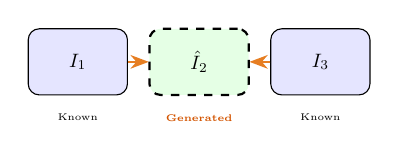
\begin{tikzpicture}[scale=0.55, every node/.style={scale=0.7}]
    \node[draw, fill=blue!10, minimum width=1.8cm, minimum height=1.2cm, rounded corners] (f1) at (0,0) {$I_1$};
    \node[draw, fill=green!10, minimum width=1.8cm, minimum height=1.2cm, rounded corners, dashed, thick] (f2) at (2.8,0) {$\hat{I}_2$};
    \node[draw, fill=blue!10, minimum width=1.8cm, minimum height=1.2cm, rounded corners] (f3) at (5.6,0) {$I_3$};
    \draw[-{Stealth}, thick, accent] (f1.east) -- (f2.west);
    \draw[-{Stealth}, thick, accent] (f3.west) -- (f2.east);
    \node[below=0.15cm, font=\tiny] at (f1.south) {Known};
    \node[below=0.15cm, color=warmaccent, font=\tiny\bfseries] at (f2.south) {Generated};
    \node[below=0.15cm, font=\tiny] at (f3.south) {Known};
\end{tikzpicture}
\end{column}
\begin{column}{0.55\textwidth}
\textbf{Why anime is uniquely challenging:}
\begin{enumerate}
    \item \textcolor{warmaccent}{\textbf{Flat color regions}} --- no texture for optical flow
    \item \textcolor{warmaccent}{\textbf{Non-linear motion}} --- characters ``pop'' between poses
    \item \textcolor{warmaccent}{\textbf{Ink line preservation}} --- thin lines blur easily
    \item \textcolor{warmaccent}{\textbf{Scene cuts}} --- abrupt shot changes
    \item \textcolor{warmaccent}{\textbf{Layer separation}} --- backgrounds pan rigidly, characters move independently
\end{enumerate}

\vspace{0.1cm}
\begin{block}{Why Deep Learning?}
\footnotesize Frames have \textbf{multi-scale spatial structure} (edges, textures, objects) and \textbf{temporal structure} (motion patterns across frames). Anime adds \textbf{layer structure}: rigid backgrounds vs.\ deformable characters. My model encodes these structural priors directly.
\end{block}
\end{column}
\end{columns}
\end{frame}

% ==============================
% Slide 3: Related Work & Novelty
% ==============================
\section{Related Work \& Novelty}

\begin{frame}{Prior Work \& My Contribution}
\begin{columns}
\begin{column}{0.48\textwidth}
\textbf{Prior Approaches:}
\vspace{0.1cm}

\scriptsize
\begin{tabular}{@{}lll@{}}
\toprule
\textbf{Method} & \textbf{Idea} & \textbf{Gap} \\
\midrule
DAIN \cite{bao2019dain} & Depth-aware flow & Not anime-specific \\
AdaCoF \cite{lee2020adacof} & Deform.\ kernels & Single motion path \\
AnimeInterp \cite{siyao2021deep} & Segment match & Ext.\ segmentation \\
RIFE \cite{huang2022rife} & Lightweight flow & Blurs heavy motion \\
LDMVFI \cite{danier2023ldmvfi} & Latent diffusion & 100$\times$ slower \\
\bottomrule
\end{tabular}

\vspace{0.2cm}
\normalsize
\footnotesize Layer decomposition dates to Wang \& Adelson (1994) \cite{wang1994layers}, but \textbf{no prior VFI method} builds anime's layer structure into the architecture.
\end{column}
\begin{column}{0.48\textwidth}
\textbf{What makes AInimotion novel:}
\begin{enumerate}
    \item \textbf{Dual-path architecture} --- dedicated BG (affine grid) + FG (AdaCoF kernels)
    \item \textbf{Domain-informed} --- encodes how anime is produced (cel layers)
    \item \textbf{Learned compositor} --- soft $\alpha$ mask, no external segmentation
    \item \textbf{Edge-aware loss} --- Sobel-weighted L1 protects ink lines
    \item \textbf{Practical} --- real-time inference ($\sim$50ms) vs.\ diffusion ($\sim$5--30s)
\end{enumerate}
\end{column}
\end{columns}
\end{frame}

% ==============================
% Slide 4: Dataset
% ==============================
\section{Dataset \& Architecture}

\begin{frame}{ATD-12K Dataset}
\begin{columns}
\begin{column}{0.5\textwidth}
\textbf{Source:} ATD-12K \cite{siyao2021deep} (CVPR 2021)

\vspace{0.2cm}
\begin{itemize}
    \item \textbf{12,000} frame triplets $(I_1, I_2, I_3)$ from \textbf{30 films}
    \item Motion categories: small, medium, \textbf{large}
    \item Established anime VFI benchmark
\end{itemize}

\vspace{0.2cm}
\textbf{Training setup:}
\begin{itemize}
    \item Random $384 \times 384$ crops
    \item Horizontal/vertical/temporal flips
    \item 100K samples per epoch
\end{itemize}
\end{column}
\begin{column}{0.45\textwidth}
\begin{block}{Why This Dataset?}
\begin{itemize}
    \item Purpose-built for anime VFI
    \item Publicly available
    \item Rich motion diversity
    \item Includes difficulty labels
\end{itemize}
\end{block}

\vspace{0.2cm}
\begin{block}{Triplet Format}
\footnotesize
$(I_1, I_2, I_3)$: $I_2$ is ground truth used as supervision during training.
\end{block}
\end{column}
\end{columns}
\end{frame}

% ==============================
% Slide 5: Architecture (user likes this)
% ==============================
\begin{frame}{Architecture Overview: LayeredInterpolator}
\begin{center}
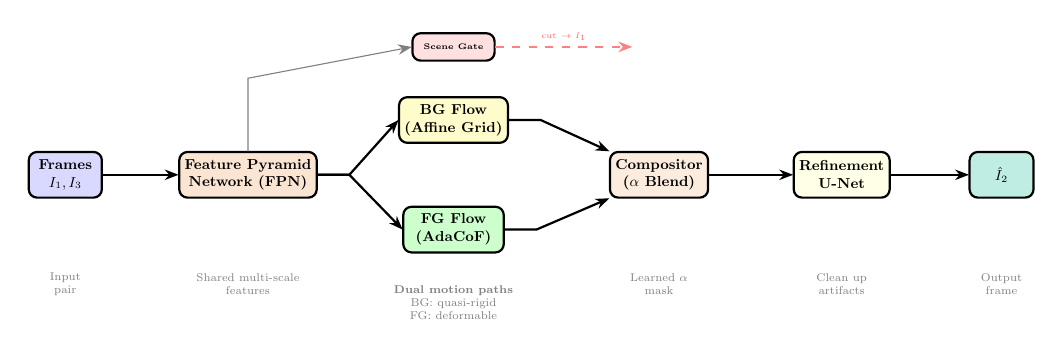
\begin{tikzpicture}[
    scale=0.58, every node/.style={scale=0.58},
    box/.style={draw, thick, rounded corners=3pt, minimum height=1cm, align=center, font=\small\bfseries},
    arr/.style={-{Stealth[length=5pt]}, thick}
]
    % --- Row 1: Main pipeline (single horizontal chain) ---
    \node[box, fill=blue!15, minimum width=1.6cm] (inputs) at (0, 0) {Frames\\$I_1, I_3$};
    \node[box, fill=accent!20, minimum width=2.4cm] (fpn) at (4, 0) {Feature Pyramid\\Network (FPN)};
    \node[box, fill=yellow!20, minimum width=2.2cm] (bg) at (8.5, 1.2) {BG Flow\\(Affine Grid)};
    \node[box, fill=green!20, minimum width=2.2cm] (fg) at (8.5, -1.2) {FG Flow\\(AdaCoF)};
    \node[box, fill=accent!15, minimum width=2cm] (comp) at (13, 0) {Compositor\\($\alpha$ Blend)};
    \node[box, fill=yellow!10, minimum width=2cm] (refine) at (17, 0) {Refinement\\U-Net};
    \node[box, fill=highlight!25, minimum width=1.4cm] (out) at (20.5, 0) {$\hat{I}_2$};

    % --- Straight arrows ---
    \draw[arr] (inputs.east) -- (fpn.west);
    \draw[arr] (fpn.east) -- ++(0.7,0) -- (bg.west);
    \draw[arr] (fpn.east) -- ++(0.7,0) -- (fg.west);
    \draw[arr] (bg.east) -- ++(0.7,0) -- (comp.north west);
    \draw[arr] (fg.east) -- ++(0.7,0) -- (comp.south west);
    \draw[arr] (comp.east) -- (refine.west);
    \draw[arr] (refine.east) -- (out.west);

    % --- Scene Gate: small label above BG ---
    \node[box, fill=red!12, minimum width=1.8cm, minimum height=0.6cm, font=\tiny\bfseries] (sg) at (8.5, 2.8) {Scene Gate};
    \draw[arr, thin, gray] (fpn.north) -- ++(0,1.6) -- (sg.west);
    \draw[arr, dashed, red!50] (sg.east) -- node[above, font=\tiny, red!60]{cut $\to I_1$} ++(3,0);

    % --- Annotations below ---
    \node[font=\scriptsize, gray, align=center] at (0, -2.4) {Input\\pair};
    \node[font=\scriptsize, gray, align=center] at (4, -2.4) {Shared multi-scale\\features};
    \node[font=\scriptsize, gray, align=center] at (8.5, -2.8) {\textbf{Dual motion paths}\\BG: quasi-rigid\\FG: deformable};
    \node[font=\scriptsize, gray, align=center] at (13, -2.4) {Learned $\alpha$\\mask};
    \node[font=\scriptsize, gray, align=center] at (17, -2.4) {Clean up\\artifacts};
    \node[font=\scriptsize, gray, align=center] at (20.5, -2.4) {Output\\frame};
\end{tikzpicture}
\end{center}
\end{frame}

% ==============================
% Slide 6: Components & Losses (merged)
% ==============================
\section{Training Strategy}

\begin{frame}{Key Components \& Loss Functions}
\begin{columns}[t]
\begin{column}{0.45\textwidth}
\textbf{Components:}
\footnotesize
\begin{itemize}
    \item \textbf{FPN:} Shared encoder, 4 scales ($\frac{1}{2}$ to $\frac{1}{16}$) + \textbf{correlation volumes} (per-pixel dot-product similarity over a $9{\times}9$ search window between frames --- tells the network ``where did each pixel move?'')
    \item \textbf{Scene Gate:} Detects hard cuts via correlation statistics, bypasses interpolation
    \item \textbf{Background:} $8\times8$ quasi-rigid affine grid for camera pans/zooms
    \item \textbf{Foreground (AdaCoF):} $9\times9$ deformable sampling kernels per pixel (81 weights + 162 offsets = 243 params/pixel)
    \item \textbf{Compositor:} Learned soft $\alpha$ mask + refinement U-Net
\end{itemize}
\end{column}
\begin{column}{0.52\textwidth}
\textbf{Generator Loss:}
\footnotesize
\[
\mathcal{L}_G = \underbrace{1.5 \cdot \mathcal{L}_{L1}}_{\text{Reconstruction}} + \underbrace{0.1 \cdot \mathcal{L}_{\text{perc}}}_{\text{VGG19}} + \underbrace{1.0 \cdot \mathcal{L}_{\text{edge}}}_{\text{Ink Lines}} + \underbrace{0.005 \cdot \mathcal{L}_{\text{GAN}}}_{\text{Phase 2}}
\]
\normalsize

\vspace{0.1cm}
\footnotesize
\begin{itemize}
    \item \textbf{$\mathcal{L}_{L1}$:} Pixel accuracy, drives PSNR
    \item \textbf{$\mathcal{L}_{\text{perc}}$:} VGG19 feature similarity, preserves style
    \item \textbf{$\mathcal{L}_{\text{edge}}$:} Sobel-weighted L1, $20\times$ multiplier on edges
    \item \textbf{$\mathcal{L}_{\text{GAN}}$:} LSGAN patch discriminator with label smoothing (0.1), Phase 2 only
\end{itemize}
\end{column}
\end{columns}
\end{frame}

% ==============================
% Slide 7: Two-Phase Training (user likes graph)
% ==============================
\begin{frame}{Two-Phase Training Strategy}
\footnotesize
\begin{columns}[t]
\begin{column}{0.46\textwidth}
\begin{block}{\centering Phase 1: Reconstruction (Ep 0--34)}
\begin{itemize}\setlength\itemsep{2pt}
    \item Generator only --- no adversarial loss
    \item $\text{lr}_G = 3 \times 10^{-4}$
    \item Loss: $\mathcal{L}_{L1} + \mathcal{L}_{\text{perc}} + \mathcal{L}_{\text{edge}}$
    \item \textbf{Goal:} PSNR $\geq$ 28 dB
\end{itemize}
\end{block}

\vspace{0.15cm}
\centering
$\Downarrow$ {\small\textit{D warmup (500 batches)}}
\vspace{0.15cm}

\begin{alertblock}{\centering Phase 2: GAN Fine-Tuning (Ep 35--49)}
\begin{itemize}\setlength\itemsep{2pt}
    \item Adversarial loss activated ($\lambda_{\text{GAN}} = 0.005$)
    \item $\text{lr}_G = 5 \times 10^{-5}$ (reduced)
    \item D trains every other batch (1:2 ratio)
    \item \textbf{Goal:} perceptual sharpness
\end{itemize}
\end{alertblock}
\end{column}
\begin{column}{0.5\textwidth}
\textbf{Why two phases?}
\begin{enumerate}\setlength\itemsep{2pt}
    \item Generator learns stable reconstructions \textit{before} seeing adversarial gradients
    \item GAN adds sharpness without destabilizing a converged generator
\end{enumerate}

\vspace{0.2cm}
\textbf{Key stabilization choices:}
\begin{itemize}\setlength\itemsep{2pt}
    \item \textbf{D warmup} --- 500 batches before G sees GAN loss
    \item \textbf{Low GAN weight} (0.005) prevents mode collapse
    \item \textbf{Adaptive $\text{lr}_D$} --- auto-adjusts based on $d_{\text{acc}}$
    \item \textbf{Label smoothing} (0.1) on discriminator
\end{itemize}
\end{column}
\end{columns}
\end{frame}

% ==============================
% Slide 8: GAN Stabilization & Infrastructure
% ==============================
\begin{frame}{GAN Stabilization \& Training Infrastructure}
\begin{columns}[t]
\begin{column}{0.48\textwidth}
\textbf{Discriminator Control:}
\begin{itemize}
    \item \textbf{D Warmup} (500 batches) --- D learns before G sees adversarial loss
    \item \textbf{Patch Discriminator} --- $70\times70$ patches, not full images
    \item \textbf{Label Smoothing} (0.1) --- prevents overconfident D
    \item \textbf{D Update Ratio} (1:2) --- D trains every other batch
    \item \textbf{Adaptive $\text{lr}_D$} --- auto-adjusts based on $d_{\text{acc}}$
\end{itemize}
\end{column}
\begin{column}{0.48\textwidth}
\textbf{Evaluation Metrics:}
\begin{itemize}
    \item \textbf{PSNR} (dB): $-10\log_{10}(\text{MSE})$. Higher = better pixel accuracy. Log scale: +3 dB $\approx$ halving MSE.
    \item \textbf{SSIM}: Measures luminance, contrast, and structural similarity ($0$--$1$). Catches distortions PSNR misses.
    \item \textbf{Visual comparison}: Side-by-side with ground truth, especially on ink lines and motion.
\end{itemize}

\vspace{0.1cm}
\begin{block}{Infrastructure}
\footnotesize
Mixed precision, grad\_clip=1.0, OOM recovery,\\
W\&B logging. RTX 5090 (32~GB VRAM).
\end{block}
\end{column}
\end{columns}
\end{frame}

% ==============================
% Slide 9: Design Evolution & Results
% ==============================
\section{Results \& Summary}

\begin{frame}{Design Evolution \& Training Progress}
\begin{columns}
\begin{column}{0.52\textwidth}
\footnotesize
\begin{tabular}{@{}lll@{}}
\toprule
\textbf{Component} & \textbf{Initial} & \textbf{Final} \\
\midrule
Base Channels & 32 & 96 ($3\times$) \\
Kernel Size & 7 & 9 (sweep winner) \\
GAN Training & From epoch 0 & Two-phase (ep 35) \\
L1 Weight & 1.0 & 1.5 (sweep-optimized) \\
GAN Weight & 0.01 & 0.005 (gentler) \\
Edge Multiplier & $10\times$ & $20\times$ (sharper) \\
Disc.\ LR & $10^{-4}$ & $2\times10^{-5}$ \\
D Update & 1:1 & 1:2 (G trains more) \\
D Warmup & None & 500 batches \\
\bottomrule
\end{tabular}

\vspace{0.15cm}
\normalsize
\textbf{Lesson:} GAN training is highly sensitive in anime VFI. The discriminator easily dominates.
\end{column}
\begin{column}{0.45\textwidth}
\textbf{Evaluation Baselines (ATD-12K):}
\footnotesize
\begin{tabular}{@{}lll@{}}
\toprule
\textbf{Method} & \textbf{PSNR} & \textbf{SSIM} \\
\midrule
RIFE & $\sim$25--27 dB & $\sim$0.85 \\
AnimeInterp & $\sim$27--29 dB & $\sim$0.88 \\
\textbf{AInimotion (target)} & \textbf{$\geq$28 dB} & \textbf{$\geq$0.90} \\
\bottomrule
\end{tabular}
\normalsize

\vspace{0.15cm}
\textbf{Sweep Results (13 experiments):}
\begin{itemize}
    \item Best: \textbf{21.80 dB} (K=9, crop 384, perc=0.1)
    \item Crop 384 alone: +0.74 dB over 256
    \item Gradients stable ($\sim 0.2$--$0.5$)
\end{itemize}

\vspace{0.1cm}
\begin{block}{Targets}
\footnotesize
Phase 1: PSNR $\geq$ 28 dB by epoch 34\\
Phase 2: + perceptual sharpness via GAN
\end{block}
\end{column}
\end{columns}
\end{frame}

% ==============================
% Slide 10: Summary & Next Steps
% ==============================
\begin{frame}{Summary \& Next Steps}
\begin{columns}
\begin{column}{0.48\textwidth}
\textbf{What I built:}
\begin{itemize}
    \item \textbf{LayeredInterpolator} --- novel dual-path architecture separating BG/FG motion
    \item \textbf{Edge-aware losses} for ink line preservation
    \item \textbf{Two-phase training} with D warmup for stable GAN integration
    \item \textbf{Robust infrastructure} --- OOM recovery, adaptive GAN balancing, mixed precision, W\&B logging
\end{itemize}
\end{column}
\begin{column}{0.48\textwidth}
\textbf{Next steps:}
\begin{itemize}
    \item Complete full 50-epoch training run
    \item Evaluate Phase 2 GAN fine-tuning
    \item Qualitative evaluation on test set
    \item Compare with RIFE, AnimeInterp baselines
\end{itemize}

\vspace{0.2cm}
\begin{block}{Project Repository}
\centering
\texttt{github.com/TWhit229/AInimotion}
\end{block}
\end{column}
\end{columns}
\end{frame}

% ==============================
% References
% ==============================
\begin{frame}[allowframebreaks]{References}
\footnotesize
\begin{thebibliography}{9}
\bibitem{siyao2021deep}
L. Siyao, S. Zhao, W. Yu, W. Sun, D. Metaxas, C. Loy, Z. Liu.
\newblock ``Deep Animation Video Interpolation in the Wild.''
\newblock \textit{CVPR}, 2021.

\bibitem{lee2020adacof}
H. Lee, T. Kim, T. Chung, D. Pak, Y. Ban, S. Lee.
\newblock ``AdaCoF: Adaptive Collaboration of Flows for Video Frame Interpolation.''
\newblock \textit{CVPR}, 2020.

\bibitem{huang2022rife}
Z. Huang, T. Zhang, W. Heng, B. Shi, S. Zhou.
\newblock ``Real-Time Intermediate Flow Estimation for Video Frame Interpolation.''
\newblock \textit{ECCV}, 2022.

\bibitem{goodfellow2014gan}
I. Goodfellow et al.
\newblock ``Generative Adversarial Nets.''
\newblock \textit{NeurIPS}, 2014.

\bibitem{mao2017lsgan}
X. Mao, Q. Li, H. Xie, R. Lau, Z. Wang, S. Smolley.
\newblock ``Least Squares Generative Adversarial Networks.''
\newblock \textit{ICCV}, 2017.

\bibitem{wang1994layers}
J. Wang, E. Adelson.
\newblock ``Representing Moving Images with Layers.''
\newblock \textit{IEEE Trans. Image Processing}, 1994.

\bibitem{bao2019dain}
W. Bao, W. Lai, C. Ma, X. Zhang, Z. Gao, M. Yang.
\newblock ``Depth-Aware Video Frame Interpolation.''
\newblock \textit{CVPR}, 2019.

\bibitem{danier2023ldmvfi}
D. Danier, F. Zhang, D. Bull.
\newblock ``LDMVFI: Video Frame Interpolation with Latent Diffusion Models.''
\newblock \textit{AAAI}, 2023.
\end{thebibliography}
\end{frame}

\end{document}
